\documentclass[10pt,a4paper]{extarticle}
\usepackage[margin=.8cm]{geometry}
\usepackage[utf8]{inputenc}
\usepackage[IL2]{fontenc}
\usepackage[czech]{babel}
\usepackage{microtype}
\usepackage{amssymb}
\usepackage{amsthm}
\usepackage{amsmath}
\usepackage{xcolor}
\usepackage{graphicx}
\usepackage{wasysym}
\usepackage{multicol}

\usepackage{tikz,pgfplots}
\pgfplotsset{compat=1.18}

\usepackage[inline]{enumitem}

\newcommand{\R}{\mathbb{R}}

\newcommand{\hint}[1]{{\color{gray}\footnotesize\noindent(Nápověda: #1)}}

\DeclareMathOperator{\tg}{tg}
\DeclareMathOperator{\cotg}{cotg}

\setlist[enumerate]{label={(\alph*)},topsep=\smallskipamount,itemsep=\smallskipamount,parsep=0pt,itemjoin={\quad}}
\setlist[itemize]{topsep=\smallskipamount,noitemsep}

\def\tisk{%
\newbox\shipouthackbox
\pdfpagewidth=2\pdfpagewidth
\let\oldshipout=\shipout
\def\shipout{\afterassignment\zdvojtmp \setbox\shipouthackbox=}%
\def\zdvojtmp{\aftergroup\zdvoj}%
\def\zdvoj{%
    \oldshipout\vbox{\hbox{%
        \copy\shipouthackbox
        \hskip\dimexpr .5\pdfpagewidth-\wd\shipouthackbox\relax
        \box\shipouthackbox
    }}%
}}%

\let\results\newpage
\let\endresults\relax

\def\resultssame{%
    \long\def\results##1\endresults{%
        %\vfill
        \noindent\rotatebox{180}{\vbox{##1}}%
    }%
}


\newtheorem*{poz}{Pozorování}

\theoremstyle{definition}
\newtheorem{uloha}{\atr Úloha}
\newtheorem{suloha}[uloha]{\llap{$\star$ }Úloha}
\newtheorem*{bonus}{Bonus}
\newtheorem*{defn}{Definice}

\pagestyle{empty}

\let\ee\expandafter

\def\vysld{}
\let\printvysl\relax
\let\printalphvysl\relax

\makeatletter

\long\def\vyslplain#1{\ee\ee\ee\gdef\ee\ee\ee\vysld\ee\c\ee{\ee\vysld\ee\printvysl\ee{\the\c@uloha}{#1}}}
\let\vysl\vyslplain

\def\locvysl#1{\ee\gdef\ee\locvysld\ee{\locvysld\item #1}}
\let\lv\locvysl

\newenvironment{ulohav}[1][]{\begin{uloha}[#1]\gdef\locvysld{\begin{enumerate*}}}{\ee\vyslplain\ee{\locvysld\end{enumerate*}}\end{uloha}}
\def\stitem{\@noitemargtrue\@item[$\star$ \@itemlabel]}

\makeatother

\def\atr{}
\def\basic{\def\atr{\llap{\mdseries$\sun$ }\gdef\atr{}}}
\def\interest{\def\atr{\llap{$\star$ }\gdef\atr{}}}
\def\iinterest{\def\atr{\llap{$\star\star$ }\gdef\atr{}}}


\begin{document}


\section*{Posuny a roztažení grafu}

Toto je graf funkce $f$.

\[\begin{tikzpicture}\begin{axis}[
        width=.6\hsize,
        grid=major,
        xmin=-8, xmax=8, xtick distance=1,
        ymin=-4, ymax=4, ytick distance=1,
        xlabel={$x$},ylabel={$y$},axis lines=middle,unit vector ratio=1 1,
        unbounded coords=discard,restrict y to domain=-40:40,samples=150]
\addplot [thick, blue, domain=0:2, smooth] {1+sqrt(1-(x-1)^2)};
\addplot [thick, blue, domain=2:4, smooth] {1-sqrt(1-(x-3)^2)};
\addplot [thick, blue] coordinates {(-8,2) (-5,1) (-2,-2) (0,1)};
\addplot [thick, blue, domain=4:4.9] {-1/(x-5)};
\addplot [thick, blue, domain=5.001:8] {ln(x-5)};
\end{axis}
\end{tikzpicture}\]

\def\emptygraph{\hbox{%
\begin{tikzpicture}\begin{axis}[
        width=.4\hsize,
        grid=major,
        xmin=-4, xmax=4, xtick distance=1,
        ymin=-4, ymax=4, ytick distance=1,
        xlabel={$x$},ylabel={$y$},axis lines=middle,unit vector ratio=1 1]
\end{axis}
\end{tikzpicture}}}

%\bigskip
\noindent
Načrtněte grafy funkcí:
\bigskip
\def\thegraph#1{\vbox{\hbox{$#1$}\smallskip\emptygraph}\hfil}

\noindent
\thegraph{f(x+1)}
\thegraph{f(x-4)}
\thegraph{f(3-x)}
\thegraph{f(2x)}
\thegraph{f(2x+1)}
\thegraph{2f(x+1)}
\thegraph{f(\frac12 x)}
\thegraph{f(\frac12 x - 1)+1}
\thegraph{f(|x|)}

\newpage

\noindent
\thegraph{f(-2x)}
\thegraph{-2f(x)}
\thegraph{-f(2x)}
\thegraph{2f(-x)}
\thegraph{f(-2x+2)}
\thegraph{-2f(-2x+2)+2}

\vfil
\hbox{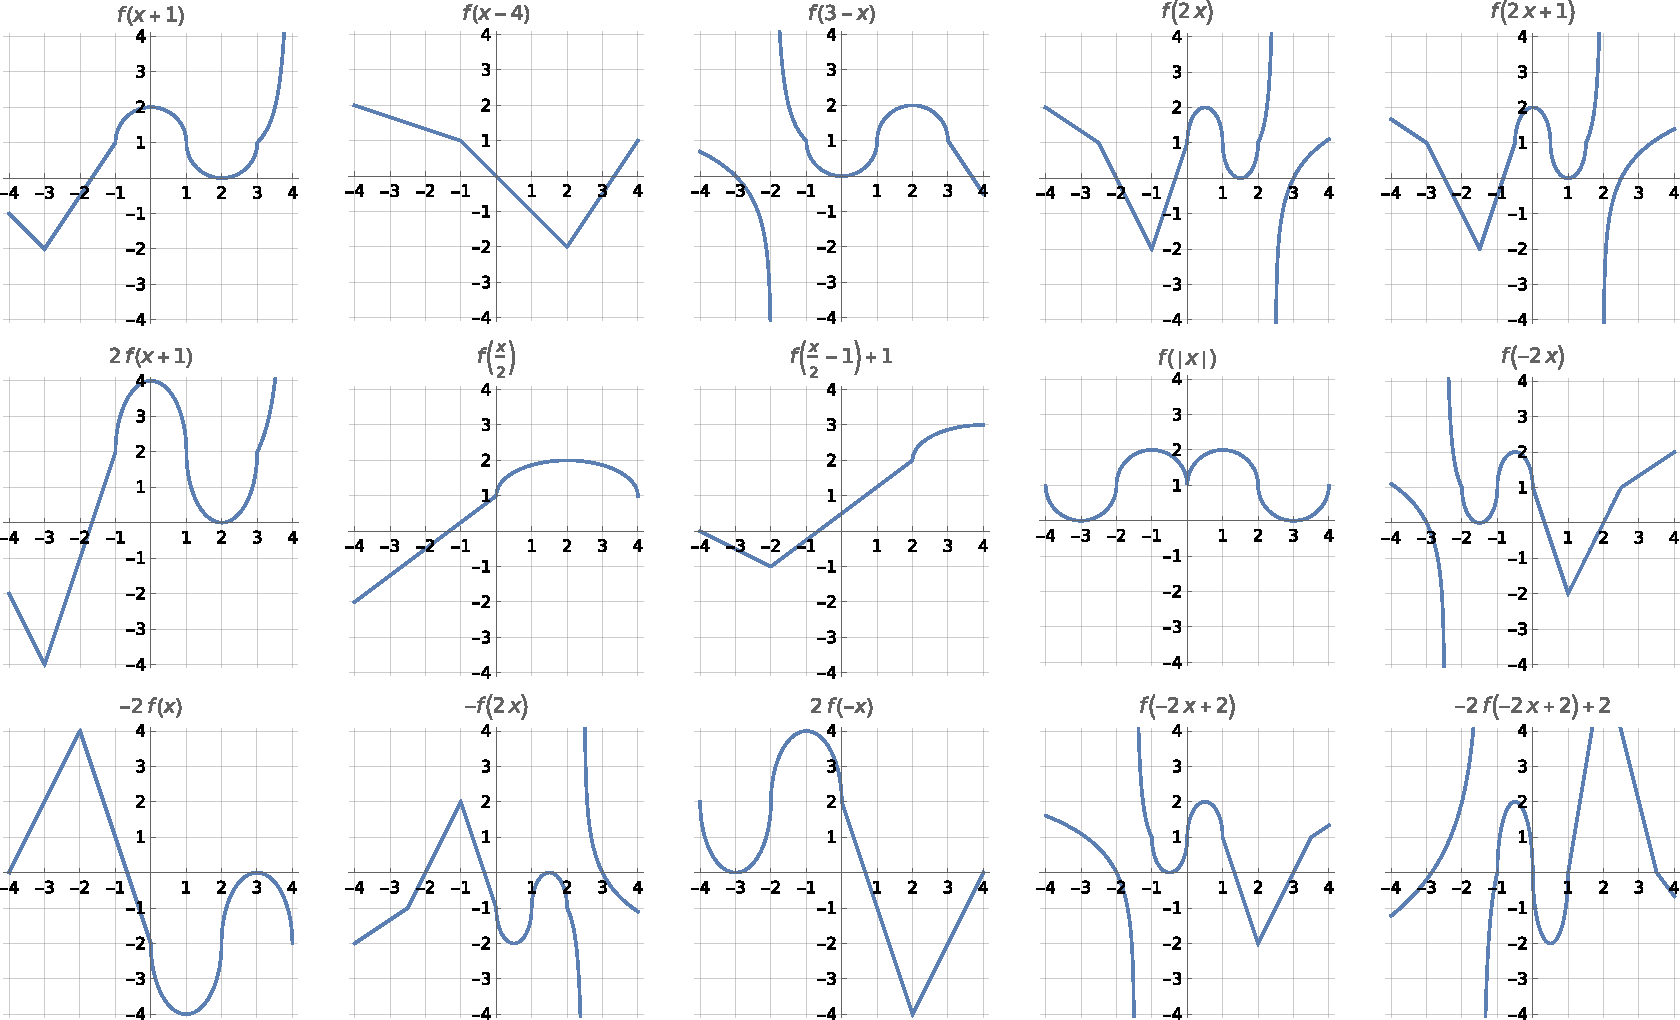
\includegraphics[width=\hsize]{grafy_3_vysl.pdf}}
\eject


\end{document}

